%!TEX root = twig.tex

\section{Multi-language Programming}
\label{sec:eval:multi-lang}

In this section, we demonstrate how Twig can be used for
multi-language programming. In a short example program, we will
show how Twig can describe typemaps that convert between three
different type systems -- C, Python, and JSON -- and how it allows
us to automatically reason about identity relationships among
them. JSON is Java-Script Object Notation, an intermediate
representation and serialization format commonly used in web
programming~\cite{json}. We describe a set of expressions similar
to the kind of typemaps found in systems such as SWIG, but which
leverage Twig's operators to build complex typemaps from simple
ones. We then show how user-defined expression reductions (see
Chapter~\ref{ch:reductions}) can be used to optimize the composed
typemaps.

Imagine that we have a Python object representing some (very)
simple personal contact information:

\begin{verbatim}
class Contact():
  def __init__(self,name,age):
    self.name = name
    self.age = age
\end{verbatim}

We would like to be able to use this object from a C program, and
we can use a typemap to perform the conversion. We can convert the
data in a number of different ways. One way is to convert the data
directly from Python to C using the Python/C
API~\cite{python-c-api}. Another way, less direct but more
flexible, is to first marshall the Python object to a JSON string
and then unmarshal the JSON into C. We might prefer to convert via
JSON if, for example, we were writing typemaps intended to work
with a variety of languages, thus avoiding the $n^2$ binding
problem described in Section~\ref{idl_discussion}.

In this example, we use the multi-language generation scheme
described in Section~\ref{sec:impl:code-gen}. First, we write some
primitive rules that unpack the object into its fields. Note that
we tell Twig that the target language in this section of code is
Python, using the \texttt{@language(Python)} directive.

\begin{verbatim}
@language(Python)

name = [contact -> py(string)] <<<
  $out = $in.name
>>>

age = [contact -> py(int)] <<<
  $out = $in.age
>>>
\end{verbatim}

The terms \texttt{py(string)} and \texttt{py(int)} represent a
string and an integer in the context of Python. The term
\texttt{contact} represents the \texttt{Contact} object defined
above.

Next, we define some primitive rules for marshalling the Python
data types in JSON. Note that for the JSON types, like
\texttt{py(json(int))}, we retain the outer \texttt{py}
constructor -- this is to indicate that the JSON string is still
represented in the context of the Python language.

\begin{verbatim}
py_int_to_json = [py(int) -> py(json(int))] <<<
  $out = int_to_json($in)
>>>

py_string_to_json = [py(string) -> py(json(string))] <<<
  $out = string_to_json($in)
>>>

py_tuple_to_json = 
  [(py(json(X)),py(json(Y))) -> py(json(pair(X,Y)))] <<<
    $out = '[' + ','.join($in1,$in2) + ']'
>>>
\end{verbatim}

The rule \texttt{py\_tuple\_to\_json} lifts a pair of JSON
objects, represented by a Twig tuple, to a pair within JSON.

Now, using these rules, we can write a more general-purpose
Python-to-JSON typemap:

\begin{verbatim}
py_to_json_step = 
  py_int_to_json | py_string_to_json | py_tuple_to_json

py_to_json = #fix(X, (#all(X) | T) ; py_to_json_step)
\end{verbatim}

The rule \texttt{py\_to\_json} uses the \texttt{\#fix} operator to
recursively convert nested tuples of Python objects to JSON.

Finally, to convert our Python \texttt{Contact} object to JSON, we
can write the following rule:

\begin{verbatim}
py_address_to_json = #fan(2);{name,age};py_to_json
\end{verbatim}

This rule sends the single contact object to a congruence
extracting the name and age, resulting in a 2-tuple of Python data
types. Then, it converts that tuple to JSON.

Next, we need primitive rules to convert from JSON into C. We use
the Jansson library~\cite{jansson} to manipulate JSON data in C.
Note that at this point we use the directive \texttt{@language(C)}
to tell Twig to use C as the target language.

\begin{verbatim}
@language(C)

json_to_tuple = [json(pair(X,Y)) -> (json(X),json(Y))] <<<
  $out1 = json_array_get($in,0);
  $out2 = json_array_get($in,1);
>>>

json_to_int = [json(int) -> int] <<<
  $out = json_int_value($in);
>>>

json_to_string = [json(string) -> string] <<<
  $out = json_string_value($in);
>>>

from_json_step = 
  json_to_int | json_to_string | json_to_tuple

from_json = #fix(X, from_json_step ; (#all(X) | T))
\end{verbatim}

Notice that, in the rules above, we are using terms like
\texttt{json(int)} to represent JSON types, rather than
\texttt{py(json(int))}. This is because in these rules, we are
working with JSON data in a C context (here, we equate the absence
the \texttt{py} constructor to indicate that the type is in C). In
both Python and C, with the libraries we chose, JSON data is
represented by a string. So, in order to move from Python to C, we
need to be able to convert a Python JSON string to a C JSON
string. The following rule accomplishes this, using the Python/C
API to convert the string.

\begin{verbatim}
py_json_to_c = [py(json(X)) -> json(X)] <<<
  json_error_t $tmp1;
  char *$tmp2 = PyString_AsString($in);
  $out = json_loads($tmp2, JSON_DECODE_ANY, &$tmp1);
>>>
\end{verbatim}

In \texttt{py\_json\_to\_c}, we use a variable \texttt{X} in the
rule's input and output pattern. In this case, we do not care what
the underlying JSON data represents, and we can convert it
regardless. This kind of polymorphism is a powerful feature of
Twig.

Putting our rules together, we can define a \texttt{main}
expression which will convert a Python \texttt{Contact} first to
JSON, and then to C.

\begin{verbatim}
main = py_address_to_json;py_json_to_c;from_json
\end{verbatim}

If we run Twig with this program on the input term
\texttt{contact} (the only term for which this program will
succeed), the output will be the tuple term \texttt{(string,int)}
representing a pair of C types. Twig will generate the following
Python code:

\begin{verbatim}
def gen1_py(in):
  x1 = in.name
  x2 = in.age
  x3 = string_to_json(x1)
  x4 = int_to_json(x2)
  x5 = tuple_to_json(x3,x4)
  return x5
\end{verbatim}

\noindent and this C code:

\begin{verbatim}
struct gen1_tuple {
  char *x1;
  int x2;
}

gen1_tuple gen1_c(PyObject *in) {
  gen1_tuple ret;
  PyObject *x1;
  char *x2;
  json_t *x3, *x4, *x5;
  char *x6;
  int x7;
  x1 = call_python("target","gen1_py",in);
  json_error_t tmp1;
  x2 = PyString_AsString(x1);
  x3 = json_loads(x2, JSON_DECODE_ANY, &tmp1);
  x4 = json_array_get(x3,0);
  x5 = json_array_get(x3,1);
  x6 = json_string_value(x4);
  x7 = json_integer_value(x5);
  ret.x1 = x6;
  ret.x2 = x7;
  return ret;
}
\end{verbatim}

The generated C function needs to return a pair of values, so we
automatically generate a C struct type for this purpose. Our
implementation currently handles this case in an ad hoc manner,
and we are working on a more robust solution.

Now, let us suppose we add some rules that leverage the Python/C
API to convert data directly, without marshaling through JSON.

\begin{verbatim}
py_string_to_c = [py(string) -> string] <<<
  $out = PyString_AsString($in);
>>>

py_int_to_c = [py(int) -> int] <<<
  $out = (int)PyInt_AsLong($in);
>>>

py_to_c_step = py_string_to_c | py_int_to_c

py_to_c = #fix(X, (py_to_c_step | #all(py_to_c_step)) ; (#all(X) | T))
\end{verbatim}

We can introduce the following expression reduction directive to
automatically replace the JSON marshaling process with calls to
the Python/C API.

\begin{verbatim}
@reduce py_to_json;json_to_c;from_json => py_to_c
\end{verbatim}

This directive exploits the isomorphic relationship between conversions from
Python to JSON, and then JSON to C, and those directly from Python to C. This
relationship is illustrated in Figure~\ref{fig:python-json-c}, where $f$, $g$,
and $h$ are Twig expressions transforming Python to JSON, JSON to C, and
Python to C, respectively. In the figure $f;g = h$, which is the relationship
we wish to exploit using an expression reduction.

\begin{figure}[ht]
\centering
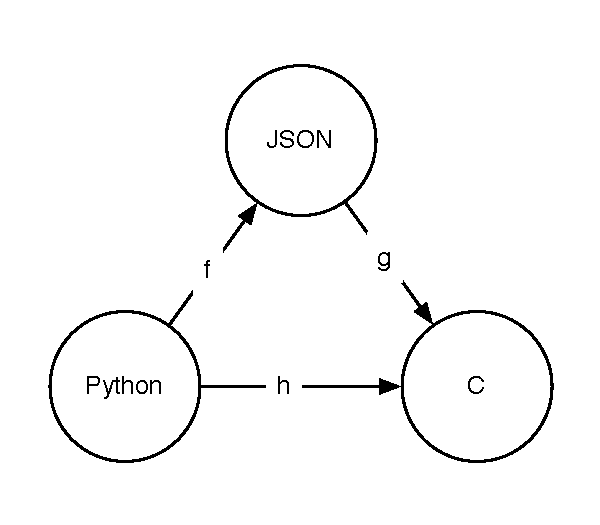
\includegraphics[width=4in]{images/python-json-c}
\caption{Typemap identities.}
\label{fig:python-json-c}
\end{figure}

The original version of \texttt{main} was

\begin{verbatim}
main = py_address_to_json;py_json_to_c;from_json
\end{verbatim}

which is equivalent to 

\begin{verbatim}
main = #fan(2);{name,age};py_to_json;py_json_to_c;from_json
\end{verbatim}

after substituting for the value of
\texttt{py\_address\_to\_json}. After applying the expression
reduction directive, \texttt{main} is rewritten to

\begin{verbatim}
main = #fan(2);{name,age};py_to_c
\end{verbatim}

Applying this new expression to the term \texttt{contact} still
yields the output term \texttt{(string,int)}, but the generated
code is much simpler and more efficient. The Python code is now:

\begin{verbatim}
def gen1_py(in):
  x1 = in.name
  return x1

def gen2_py(in):
  x1 = in.age
  return x1
\end{verbatim}

\noindent and the C code is:

\begin{verbatim}
gen1_tuple gen1_c(PyObject *in) {
  gen1_tuple ret;
  PyObject *x1,*x2;
  char *x3;
  int x4;
  x1 = call_python("target","gen1_py",in);
  x2 = call_python("target","gen2_py",in);
  x3 = PyString_AsString(x1);
  x4 = (int)PyInt_AsLong(x2);
  ret.x1 = x3;
  ret.x2 = x4;
  return ret;
}
\end{verbatim}

It is notable that systems such as SWIG, based on monolithic
typemaps, could not perform reductions of this kind. This is
because, unlike Twig expressions, monolithic typemaps have no
structure that SWIG can rewrite.
